\documentclass[chaptersright]{informeutn}
\usepackage[utf8]{inputenc}
\usepackage{array}
\usepackage{geometry}
\usepackage[table]{xcolor}
\usepackage{colortbl}
\usepackage{caption}
\usepackage{graphicx}
\usepackage{amsmath}
\usepackage{multirow}
\usepackage{float}

\materia{Dispositivos Electronicos I}
\titulo{Trabajo Practico N°3: Transistores Bipolares (BJT)}
\comision{3R2}
\autores{Documentador y operador: Angelo Prieto 401012\\ Coordinador: Gaston Grasso 401892}
\fecha{24-06-2025}

\begin{document}
\maketitle
\tableofcontents

\chapter{Introduccion}
El transistor bipolar de unión (BJT) es un 
dispositivo semiconductor fundamental en la electrónica analógica, 
ampliamente utilizado en aplicaciones de amplificación y conmutación. El 
presente trabajo práctico tiene como finalidad estudiar el comportamiento 
del transistor NPN bajo diferentes configuraciones y condiciones de 
polarización, con el objetivo de comprender su funcionamiento interno y 
su respuesta en cada zona de operación (zona activa, de saturación y de 
corte).

La metodología empleada combina el análisis teórico del circuito, 
simulaciones por software y la posterior implementación en laboratorio. 
Este enfoque permite analizar el comportamiento del transistor 
en función de sus condiciones de operación, validar los modelos teóricos 
mediante simulación y contrastar los resultados con mediciones reales. 
Este trabajo se centrará en el estudio del transistor NPN, mientras que
el análisis del transistor PNP será complementado en aula según los
objetivos establecidos en las consignas.

A través de este trabajo se busca fortalecer la comprensión de los 
mecanismos de conducción en dispositivos semiconductores, y sentar las 
bases para el diseño y análisis de circuitos electrónicos más complejos.

\chapter{Identificación de las zonas de trabajo del transistor}
En esta sección se analiza el comportamiento del transistor NPN en sus 
distintas regiones de operación: corte, activa y saturación. Para ello, 
se polarizan los circuitos de diferentes maneras, observando las 
relaciones entre tensiones y corrientes que caracterizan cada zona de 
trabajo.

Previo a la implementación práctica en el laboratorio, se realizaron 
simulaciones que permitieron anticipar el comportamiento esperado del 
transistor bajo cada condición de polarización. Esto facilitó la 
identificación de los parámetros clave a medir y la interpretación de los 
resultados obtenidos.

\section{Zona de corte}
  \subsection{Actividad de simulación}
    Se parte analizando el comportamiento del transistor NPN cuando 
    se encuentra en la región de corte. Para ello, se simula un 
    circuito en el cual la juntura base-emisor no se encuentra 
    polarizada directamente, impidiendo el flujo de corriente desde 
    la base. Sin embargo, la juntura colector-emisor sí está 
    polarizada, lo que permite observar que, en ausencia de 
    corriente de base, el transistor no conduce corriente de 
    colector significativa.

    Esta condición representa el estado "apagado" del transistor, 
    equivalente al de un interruptor abierto. El análisis de esta 
    región permite confirmar que, sin polarización directa en la 
    base, el transistor permanece en corte, aún cuando exista una 
    tensión entre colector y emisor.
    \begin{figure}[H]
        \centering
        \includegraphics[width=0.8\textwidth, keepaspectratio]{pictures/circuito-simulacion-corte.png}
        \caption{}
    \end{figure}
    \begin{figure}[H]
        \centering
        \includegraphics[width=0.8\textwidth, keepaspectratio]{pictures/curva-simulacion-corte.png}
        \caption{$I_B$ en función de $V_{BE}$ resultado de simulación
        ~\ref{fig:circuito-simulacion-corte}}
    \end{figure}

  A partir de la simulación y la curva obtenida, se puede concluir
  que al no estar polarizada la juntura base-emisor, por el transistor
  circula una corriente muy pequeña, denominada corriente de fuga en
  el colector $I_{CEO}$ (en este caso, $I_{CEO}\approx26pA$), debido a 
  los portadores minotarios. Por lo general, esta corriente es 
  despreciable, así que se puede decir que al no estar polarizada la
  juntura base-emisor (y si la juntura colector-base), el transistor
  se encuentra en la zona de corte y no circula
  corriente por el mismo ($I_C = 0$).
  
  \section{Polarizacion de la juntura Base-Emisor}
    Con esta actividad se busca caracterizar el comportamiento de la
    juntra base-emisor del transistor. Esto es fundamental ya que en
    cualquier aplicación del transistor, sea como amplificador o
    dispositivo de conmutación, se requiere una correcta polarización
    de la juntura en cuestión.
    
    \subsection{Actividad de simulación}
    Se comenzó simulando el circuito de la figura ~\ref{fig:circuito-simulacion-pol-junt-BE} en la aplicación de simulación
    \textit{LTSpice}. Se puede observar que para esta simulación, se
    mantiene la fuente $V_2 (V_{CC})$ constante, y la curva obtenida
    es la corriente de base $I_B$ en función de la tensión $V_1(V_{BB})$, la cual se hace variar, o se hace un barrido, de 0V a 10V.
    Luego, se plantean dos simulaciones más para el mismo circuito, 
    pero esta vez haciendo variar $V_2 (V_{CC})$ (simulación 
    ~\ref{fig:circuito-simulacion-pol-junt-BE-variandoVCC}) y haciendo
    variar la temperatura (simulación ~\ref{fig:circuito-simulacion-pol-junt-BE-variandoTEMP}).

    \begin{figure}[H]
        \centering
        \includegraphics[width=1\textwidth, keepaspectratio]{pictures/circuito-simulacion-pol-junt-BE.png}
        \caption{Circuito polarización de juntura BE para $V_{CC} = 10V$ simulado en LTSpice}
        \label{fig:circuito-simulacion-pol-junt-BE}
    \end{figure}

    \begin{figure}[H]
        \centering
        \includegraphics[width=1\textwidth, keepaspectratio]{pictures/curva-simulacion-pol-junt-be.png}
        \caption{$I_B$ en función de $V_{BE}$ resultado de simulación
        ~\ref{fig:circuito-simulacion-pol-junt-BE}}
    \end{figure}

    \begin{figure}[H]
        \centering
        \includegraphics[width=1\textwidth, keepaspectratio]{pictures/circuito-simulacion-pol-junt-BE-variandoVCC.png}
        \caption{Circuito polarización de juntura BE variando $V_{CC}$ simulado en LTSpice}
        \label{fig:circuito-simulacion-pol-junt-BE-variandoVCC}
    \end{figure}

    \begin{figure}[H]
        \centering
        \includegraphics[width=1\textwidth, keepaspectratio]{pictures/curva-simulacion-pol-junt-be-variandoVCC.png}
        \caption{$I_B$ en función de $V_{BE}$ resultado de simulación
        ~\ref{fig:circuito-simulacion-pol-junt-BE-variandoVCC}}
    \end{figure}

    \begin{figure}[H]
        \centering
        \includegraphics[width=1\textwidth, keepaspectratio]{pictures/circuito-simulacion-pol-junt-be-variandoTEMP.png}
        \caption{Circuito polarización de juntura BE variando la temperatura simulado en LTSpice}
        \label{fig:circuito-simulacion-pol-junt-BE-variandoTEMP}
    \end{figure}

    \begin{figure}[H]
        \centering
        \includegraphics[width=1\textwidth, keepaspectratio]{pictures/curva-simulacion-pol-junt-be-variandoTEMP.png}
        \caption{$I_B$ en función de $V_{BE}$ resultado de simulación 
        ~\ref{fig:circuito-simulacion-pol-junt-BE-variandoTEMP}}
    \end{figure}
    
    \subsection{Actividad de laboratorio}
    Luego de realizar las simulaciones y entendiendo el comportamiento del
    transistor al polarizar la juntura base-emisor, se procedió a ensayar el
    modelo \textit{BC547B} en el laboratorio central de la facultad. Para ello,
    se armó el mismo circuito simulado en una placa de pruebas, con los mismos
    valores de resistores utilizados en la simulación ($R_B = 10k\Omega$ y
    $R_C = 560\Omega$). Se utilizó también dos fuentes de alimentación, una fija
    ($V_{CC}=10V$) y una que se hizo variar de 0V a 10V ($V_{BB}$). De este modo,
    se registró los distintos valores de corriente de base $I_B$ y tensión
    base-emisor $V_{BE}$ obtenidos, los cuales se registró en la siguiente tabla
    y obteniendo la respectiva curva:
    
      \begin{center}
      \resizebox{\textwidth}{!}{%
        \begin{tabular}{|c|c|c|c|c|c|c|c|c|c|c|c|}
          \hline
          \textbf{$V_{BB}$} & \textbf{0} & \textbf{0.284V} & \textbf{0.393V} & \textbf{0.5V}
          & \textbf{0.596V} & \textbf{0.7V} & \textbf{0.8V} & \textbf{1.06V} & \textbf{3V} & \textbf{7V} & \textbf{10V} \\
          \hline
          $I_B$ & 0 A & 29 nA & 43 nA & 91 nA & 0.78 uA & 4.99 uA & 12.46 uA & 35.84 uA & 226.3 uA & 625 uA & 929 uA \\
          \hline
          $V_{BE}$ & 0 V & 0.27 V & 0.38 V & 0.48 V & 0.57 V & 0.63 V & 0.66 V & 0.68 V & 0.73 V & 0.75 V & 0.75 V \\
          \hline
        \end{tabular}%
      }
      \end{center}

    \begin{figure}[H]
        \begin{tikzpicture}
          \begin{axis}[
            axis lines = left,
            ylabel = {$I_{B}[A]$},
            xlabel = {$V_{BE}[V]$},
            ymin=0, ymax=0.001,
            xmin=0, xmax=0.9,
            width=15cm,
            height=7cm,
            clip=false,
          ]
            \addplot[
              color=blue,
              mark=*,
              only marks,
              mark options={scale=1.3}
            ]
            coordinates {
                (0.00, 0)
                (0.27, 29e-9)
                (0.38, 43e-9)
                (0.48, 91e-9)
                (0.57, 0.78e-6)
                (0.63, 4.99e-6)
                (0.66, 12.46e-6)
                (0.68, 35.84e-6)
                (0.73, 226.3e-6)
                (0.75, 625e-6)
                (0.75, 929e-6)
            };
            \addplot[
              color=blue,
              thick
            ]
            coordinates {
                (0.00, 0)
                (0.27, 29e-9)
                (0.38, 43e-9)
                (0.48, 91e-9)
                (0.57, 0.78e-6)
                (0.63, 4.99e-6)
                (0.66, 12.46e-6)
                (0.68, 35.84e-6)
                (0.73, 226.3e-6)
                (0.75, 625e-6)
                (0.75, 929e-6)
            };
          \end{axis}
        \end{tikzpicture}
        \caption{\footnotesize $I_B$ en función de $V_{BE}$ a partir de mediciones en laboratorio}
        \end{figure}

        \subsubsection{Fotografías}
        A continuación se presentan fotografías de los distintos instrumentos de
        medición y energización, y la disposición del cicuito ensayado:

        \begin{figure}[H]
        \begin{minipage}{0.40\textwidth}
          \centering
          \includegraphics[width=\textwidth]{pictures/disposicion-juntura-be.jpeg}
          \caption{Circuito implementado en placa de pruebas.}
          \label{fig:disposicion-juntura-be}
        \end{minipage}
        \hfill
        \begin{minipage}{0.40\textwidth}
          \centering
          \includegraphics[width=\textwidth]{pictures/fuente1.jpeg}
          \caption{Fuente 1 fija ($V_{CC}=10V$).}
          \label{fig:fuente1}
        \end{minipage}
        \vspace{0.5cm} % espacio vertical entre filas
        \begin{minipage}{0.40\textwidth}
          \centering
          \includegraphics[width=\textwidth]{pictures/fuente2.jpeg}
          \caption{Fuente 2 variable ($0< V_{BB}<10V$).}
          \label{fig:fuente2}
        \end{minipage}
        \hfill
        \begin{minipage}{0.40\textwidth}
          \centering
          \includegraphics[width=\textwidth]{pictures/multimetros-juntura-be.jpeg}
          \caption{Multimetros utilizados. Multímetro derecha: marca UNI-T modelo UT61D+. Multímetro medio: marca genérica modelo DT9205A. Multímetro izquierda: marca BRYMEN modelo BM837RS.}
          \label{fig:multimetros}
        \end{minipage}
        \end{figure}

        \subsubsection{Conclusión}

          Se puede observar en la simulación que cuando no se le inyecta corriente a la base la unica corriente que
          persiste en el dispositivo es la de fuga, que esta en el orden de los pico-amperes. Por otro lado se puede
          observar como la juntura BE, al ser polarizada, se comporta como un diodo (por que al final es eso), tanto en
          la curva de corriente como en la variacion de la misma por efectos de la temperatura del dispositivo.
        
\chapter{Curvas características}
El objetivo de esta actividad es analizar las curvas características de salida del transistor, es decir, cómo varía la corriente de colector $I_C$ en función de la tensión colector-emisor $V_{CE}$ para distintos valores de corriente de base $I_B$. Estas curvas permiten visualizar el comportamiento del transistor en sus diferentes regiones de operación (corte, activa y saturación) y son fundamentales para comprender su funcionamiento como dispositivo de control de corriente.

A través del trazado de estas curvas, se puede observar cómo el transistor responde a cambios en la polarización, identificar los límites entre las distintas zonas de trabajo y evaluar su ganancia en región activa. Previamente al ensayo en el laboratorio, se realizaron simulaciones para predecir el comportamiento esperado y facilitar la comparación con los resultados experimentales.

Este análisis resulta esencial para el diseño y la elección del punto de operación (punto Q) en aplicaciones de amplificación o conmutación.

  \section{Actividad de simulación}
  Primero, se procede a simular el circuito de la figura 
  ~\ref{fig:circuito-simulacion-salida}, la cual se puede observar que se hace
  un barrido de $V_2(V_{CC})$, para distintas tensiones de $V_1(V_{BB)}$. Las
  distintas curvas resultantes se pueden observar en la figura ~\ref{fig:curva-simulacion-salida}
      \begin{figure}[H]
          \centering
          \includegraphics[width=1\textwidth, keepaspectratio]{pictures/circuito-simulacion-salida.png}
          \caption{Circuito emisor-común con fuentes variables para observar curva característica del transistor simulado en LTSpice}
          \label{fig:circuito-simulacion-salida}
      \end{figure}
  
      \begin{figure}[H]
          \centering
          \includegraphics[width=1\textwidth, keepaspectratio]{pictures/curva-simulacion-salida.png}
          \caption{$I_C$ en función de $V_{CE}$ resultado de simulación 
          ~\ref{fig:circuito-simulacion-salida}}
          \label{fig:curva-simulacion-salida}
      \end{figure}

  \section{Actividad de laboratorio}
  Luego de realizar la simulación, se procedió a armar el mismo circuito
  en la placa de pruebas, utilizando los mismos valores resisistivos y el
  mismo criterio para las fuentes de alimentación. Los valores obtenidos
  se registraron en la tabla que se ve a continuación, y luego se trazaron
  las respectivas curvas.
    
    \begin{table}[H]
    \centering
    \resizebox{\textwidth}{!}{%
    \begin{tabular}{|c|c|c|c|c|c|c|c|c|c|c|}
      \hline
      \multirow{2}{*}{$V_{CC}$ [V]} & 
      \multicolumn{2}{|c|}{$I_B=0\,\text{A}$} & 
      \multicolumn{2}{|c|}{$I_B=10\,\mu\text{A}$} & 
      \multicolumn{2}{|c|}{$I_B=15\,\mu\text{A}$} & 
      \multicolumn{2}{|c|}{$I_B=20\,\mu\text{A}$} & 
      \multicolumn{2}{|c|}{$I_B=25\,\mu\text{A}$} \\
      \cline{2-11}
       & $I_C$ & $V_{CE}$ & $I_C$ & $V_{CE}$ & $I_C$ & $V_{CE}$ & $I_C$ & $V_{CE}$ & $I_C$ & $V_{CE}$ \\
      \hline
      0    &  0 A  &  0 V      &  0 A        &  0 V     &  0 A       &  0 V      &  0 A      &  0 V     &  0 A       &   0 V    \\
      0.25 &  0  A &  0.24 V   &  312.5 uA   &  0.06 V  &  325 uA    &  0.05 V   &  332 uA   &  0.05 V  &  333 uA    &   0.04 V \\
      0.5  &  0  A &  0.48 V   &  701.7 uA   &  0.09 V  &  737 uA    &  0.08 V   &  725 uA   &  0.07 V  &  764 uA    &   0.06 V \\
      1    &  0  A &  0.99 V   &  1.564 mA   &  0.12 V  &  1.58 mA   &  0.11 V   &  1.64 mA  &  0.1 V   &  1.7 mA    &   0.09 V \\
      2    &  0  A &  2 V      &  3.125 mA   &  0.21 V  &  3.32 mA   &  0.15 V   &  3.36 mA  &  0.13 V  &  3.37 mA   &   0.12 V \\
      5    &  0  A &  5 V      &  2.84 mA    &  3.41 V  &  4.04 mA   &  2.67 V   &  5.49 mA  &  1.96 V  &  7.9 mA    &   0.51 V \\
      10   &  0  A &  9.97 V   &  2.97 mA    &  8.32 V  &  4.37 mA   &  7.53 V   &  5.85 mA  &  6.58 V  &  8.43 mA   &   5.23 V \\
      \hline
    \end{tabular}
    }
    
    \end{table}
    
    \begin{figure}[H]
    \centering
    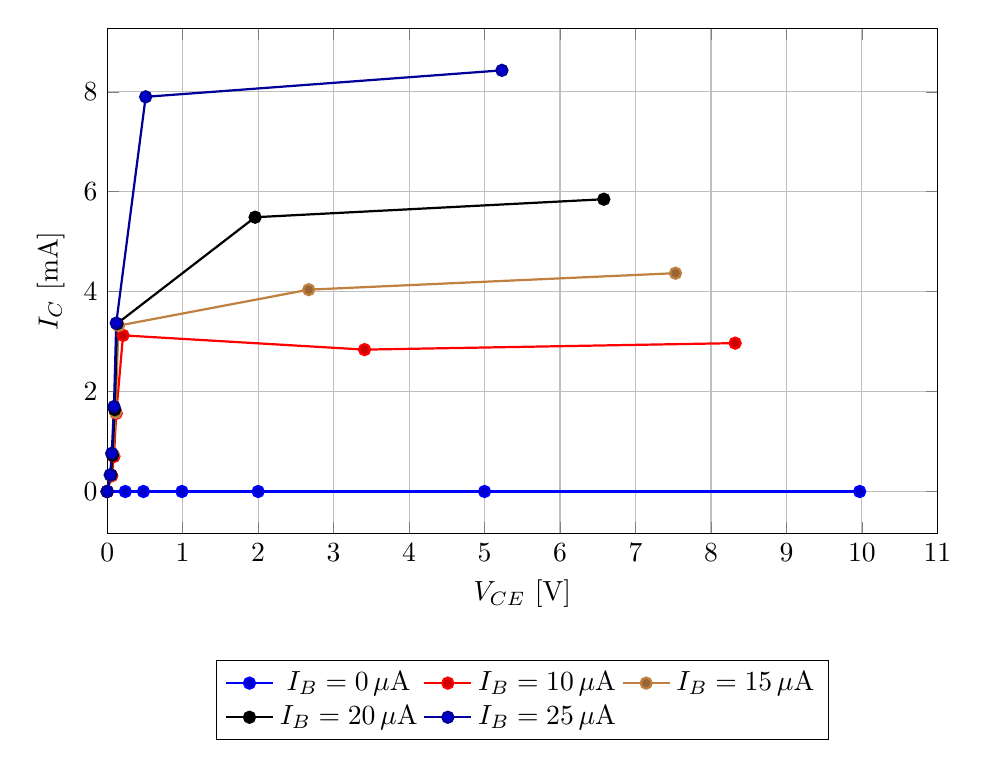
\begin{tikzpicture}
    \begin{axis}[
        width=\textwidth,
        height=8cm,
        xlabel={$V_{CE}$ [V]},
        ylabel={$I_C$ [mA]},
        grid=both,
        xmin=0, xmax=11, % <-- extendido para que entre todo
        legend style={at={(0.5,-0.25)}, anchor=north, legend columns=3},
    ]
    
    \addplot+[mark=*, thick, blue] coordinates {
      (0,0) (0.24,0) (0.48,0) (0.99,0) (2,0) (5,0) (9.97,0)
    };
    \addlegendentry{$I_B = 0\,\mu$A}
    
    \addplot+[mark=*, thick, red] coordinates {
      (0,0) (0.06,0.3125) (0.09,0.7017) (0.12,1.564) (0.21,3.125) (3.41,2.84) (8.32,2.97)
    };
    \addlegendentry{$I_B = 10\,\mu$A}
    
    \addplot+[mark=*, thick, brown] coordinates {
      (0,0) (0.05,0.325) (0.08,0.737) (0.11,1.58) (0.15,3.32) (2.67,4.04) (7.53,4.37)
    };
    \addlegendentry{$I_B = 15\,\mu$A}
    
    \addplot+[mark=*, thick, black] coordinates {
      (0,0) (0.05,0.332) (0.07,0.725) (0.10,1.64) (0.13,3.36) (1.96,5.49) (6.58,5.85)
    };
    \addlegendentry{$I_B = 20\,\mu$A}
    
    \addplot+[mark=*, thick, blue!60!black] coordinates {
      (0,0) (0.04,0.333) (0.06,0.764) (0.09,1.7) (0.12,3.37) (0.51,7.9) (5.23,8.43)
    };
    \addlegendentry{$I_B = 25\,\mu$A}
    
    \end{axis}
    \end{tikzpicture}
    \caption{Curvas de salida del \textit{BC547B} para distintas $I_B$}
    \end{figure}
    
    \begin{figure}[H]
          \centering
          \includegraphics[width=0.4\textwidth, keepaspectratio, angle=90]{pictures/disposicion-curvas-salida.jpeg}
          \caption{Disposición circuito implementado para ensayo en laboratorio.}
    \end{figure}

    \subsubsection{Conclusión}
      Se observó que un aumento en la corriente de base ($I_B$) produce un incremento proporcional en la corriente de
      colector ($I_C$), evidenciando el comportamiento típico del transistor en la región activa, donde 
      $I_C \approx h_{FE} \cdot I_B$. Por lo tanto, la base actúa como un control de paso para la corriente de colector,
      funcionando de forma análoga a una llave controlada por corriente.

\chapter{Caracteristicas de transferencia de corriente}
En esta sección se analiza la relación entre la corriente de colector $I_C$ y 
la corriente de base $I_B$ del transistor NPN, conocida como ganancia de 
corriente continua o $\beta$. Esta relación es fundamental para el diseño de
circuitos amplificadores y puede variar según el punto de operación y las
características del dispositivo.

A través de una práctica de laboratorio, se medirá en distintas condiciones
de polarización para observar si $\beta$ se mantiene constante en las diferentes
regiones de trabajo del transistor. Previamente, se realizaron simulaciones
que permitieron anticipar el comportamiento esperado y facilitar la
comparación con los resultados experimentales.

  \section{Actividad de simulación}
  Como se realizó a lo largo de todo este trabajo práctico, antes de realizar
  los ensayos en el laboratorio, se realiza la simulación del circuito a
  ensayar. En la figura \ref{fig:circuito-simulacion-beta} se presenta el
  circuito y los parámetros de simulación, y en la figura
  \ref{fig:curva-simulacion-beta} se presentan las curvas resultantes.
        \begin{figure}[H]
          \centering
          \includegraphics[width=\textwidth, keepaspectratio]{pictures/circuito-simulacion-beta.png}
          \caption{Circuito implementado en la simulación.}
          \label{fig:circuito-simulacion-beta}
      \end{figure}
  
      \begin{figure}[H]
          \centering
          \includegraphics[width=1\textwidth, keepaspectratio]{pictures/curva-simulacion-beta.png}
          \caption{$I_C$ en función de $I_B$ resultado de simulación 
          ~\ref{fig:circuito-simulacion-beta}}
          \label{fig:curva-simulacion-beta}
      \end{figure}

  \section{Actividad de laboratorio}
  Posterior a la simulación, se procede a implementar el mismo circuito en una
  placa de pruebas y se realizan las distintas mediciones, las cuales fueron
  registradas en la tabla \ref{fig:tabla-beta} y luego se trazaron las curvas
  correspondientes.
    \begin{table}[H]
      \centering
      \begin{tabular}{|c|c|c|c|}
        \hline
        $I_B$ [$\mu$A] & $I_C$ (@$V_{CE\text{(inicial)}}$ = 2 V) & $I_C$ (@$V_{CE\text{(inicial)}}$ = 5 V) & $I_C$ (@$V_{CE\text{(inicial)}}$ = 8 V) \\
        \hline
        5  & 1.66 mA & 1.85 mA & 2.46 mA \\
        7  & 2.17 mA & 2.44 mA & 2.5 mA  \\
        10 & 3.14 mA & 3.5 mA  & 3.6 mA  \\
        20 & 6.53 mA & 6.98 mA & 7.4 mA  \\
        \hline
      \end{tabular}
      \caption{Valores registrados del ensayo en laboratorio}
      \label{fig:tabla-beta}
    \end{table}


    \begin{figure}[H]
      \centering
      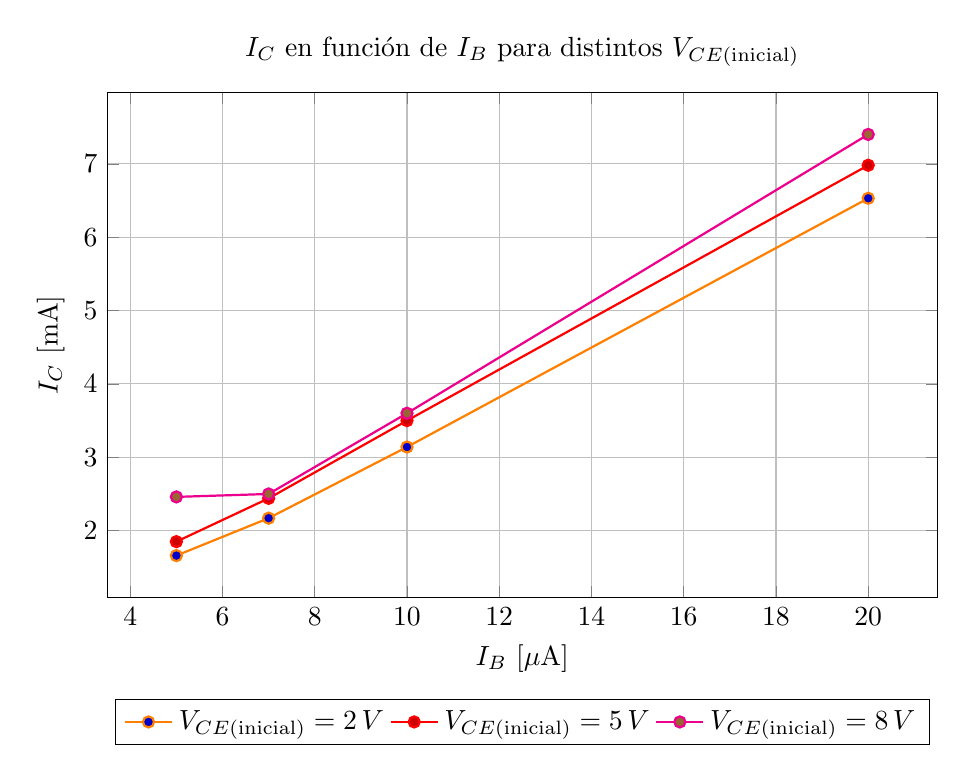
\begin{tikzpicture}
      \begin{axis}[
          width=\textwidth,
          height=8cm,
          xlabel={$I_B$ [$\mu$A]},
          ylabel={$I_C$ [mA]},
          grid=both,
          legend style={at={(0.5,-0.2)}, anchor=north, legend columns=3},
          title={$I_C$ en función de $I_B$ para distintos $V_{CE(\text{inicial})}$}
      ]
      
      \addplot+[mark=*, thick, orange] coordinates {
        (5,1.66) (7,2.17) (10,3.14) (20,6.53)
      };
      \addlegendentry{$V_{CE(\text{inicial})} = 2\,V$}
      
      \addplot+[mark=*, thick, red] coordinates {
        (5,1.85) (7,2.44) (10,3.5) (20,6.98)
      };
      \addlegendentry{$V_{CE(\text{inicial})} = 5\,V$}
      
      \addplot+[mark=*, thick, magenta] coordinates {
        (5,2.46) (7,2.5) (10,3.6) (20,7.4)
      };
      \addlegendentry{$V_{CE(\text{inicial})} = 8\,V$}
      
      \end{axis}
      \end{tikzpicture}
      \caption{Curvas $I_C$ en función de $I_B$ para distintos $V_{CE(\text{inicial})}$}
    \end{figure}

    \begin{table}[H]
      \centering
      \begin{tabular}{|c|c|c|c|c|}
      \hline
      $V_{CE(\text{inicial})}$ & $\beta$ @ $I_B=5\,\mu$A & $I_B=7\,\mu$A & $I_B=10\,\mu$A & $I_B=20\,\mu$A \\
      \hline
      2 V  & 332   & 310    & 314   & 326.5 \\
      5 V  & 370   & 348.6  & 350   & 349   \\
      8 V  & 492   & 357.1  & 360   & 370   \\
      \hline
      \end{tabular}
      \caption{Valores de $\beta = \frac{I_C}{I_B}$ para distintos $V_{CE(\text{inicial})}$}
    \end{table}

   \subsubsection{Fotografías}
    A continuación se adjunta una fotografía de la disposición del circuito
    ensayado para esta actividad. Las fuentes de alimentación y los elementos
    de medición empleados son los mismos que se emplearon en las secciones
    anteriores.

    \begin{figure}[H]
        \centering
        \includegraphics[width=0.6\textwidth, keepaspectratio]{pictures/disposicion-beta.jpeg}
        \caption{Fotografía del ensayo realizado para esta actividad}
    \end{figure}

    \subsubsection{Conclusión}
     En este ejercicio nos dimos cuenta de que cometimos el error de ajustar la tensión colector-emisor a su valor 
     inicial en cada medición, en lugar de dejar que variara naturalmente. Esto provocó que obtuviéramos una curva 
     lineal, en lugar de la curva característica del transistor observada en la simulación. Gracias a esta herramienta,
     pudimos identificar nuestro error y comprender la importancia de contar con simulaciones para verificar el 
     comportamiento de los circuitos, especialmente cuando los resultados experimentales no coinciden con lo esperado.

     Por otro lado, la simulación también nos permitió visualizar cómo la corriente de colector depende directamente
     tanto de la corriente inyectada a la base como de la tensión colector-emisor, reafirmando el funcionamiento típico
     del transistor en sus distintas regiones de operación.

\chapter{Interpretacion de las especificaciones del fabricante}

\section{Significado de cada parametro del datasheet}


\subsubsection{Características eléctricas a $25^\circ$C }

\begin{tabular}{p{7cm} p{7cm}}
    $V_{(BR)CEO}$ : Tensión de ruptura colector-emisor con base abierta. Es el voltaje máximo que puede haber entre colector y emisor cuando la base está abierta, sin que el transistor se dañe. &
    $h_{FE}$ : Ganancia de corriente en continua. También conocido como $\beta$, es la relación entre la corriente de colector y la de base ($I_C/I_B$). \\
    
    $I_{CEO}$ : Corriente de fuga colector-emisor con base abierta. Es una corriente no deseada que circula aunque no se esté polarizando el transistor. &
    $h_{fe}$ : Igual que $h_{FE}$ pero en pequeña señal. \\
    
    $I_{CES}$ : Corriente de fuga colector-emisor con base en corto a emisor. También es una corriente de fuga, pero ahora con la base conectada a emisor. &
    $V_{BE}$ : Tensión base-emisor directa. Es el voltaje que hay que aplicar entre base y emisor para que el transistor conduzca (usualmente $\sim$0.6–0.7V en BJT de silicio). \\
    
    $I_C$ : Corriente máxima de colector. Es la corriente máxima que el transistor puede manejar por el colector sin dañarse. &
    $V_{CE(\text{sat})}$ : Tensión de saturación colector-emisor. Es el voltaje que queda entre colector y emisor cuando el transistor está completamente saturado. \\
    
    $I_{EBO}$ : Corriente de fuga emisor-base con colector abierto. Otra corriente de fuga, esta vez desde emisor hacia base. &
    $P_d$ : Potencia disipada máxima. Es la cantidad de potencia que el transistor puede disipar en forma de calor sin dañarse. \\
\end{tabular}

\vspace{1em}
\subsubsection{Características térmicas}

\begin{tabular}{p{14cm}}
    $\theta_{jc}$ : Resistencia térmica unión-colector. Cuánto se eleva la temperatura de la unión por cada watt que se disipa hacia el colector. (°C/W) \\
    $\theta_{ja}$ : Resistencia térmica unión-ambiente. Qué tan eficiente es el transistor para disipar calor al aire sin disipador. (°C/W) \\
\end{tabular}

\vspace{1em}
\subsubsection{Características de conmutación a $25^\circ$C}

\begin{tabular}{p{14cm}}
    $t_{on}$ : Tiempo de encendido. Es el tiempo que tarda el transistor en pasar de apagado a encendido (conducción). \\
\end{tabular}

  \section{Relevamiento para distintos transistores}

    \subsection{BC548}
  
    \subsubsection{Características eléctricas a $25^\circ$C}
    \begin{tabular}{ll}
    $V_{(BR)CEO} = 30 \V$         & \hspace{2cm} $h_{FE} =$ min 110, max 800 \\
    $I_{CEO} = $ No esta en el DS           & \hspace{2cm} $h_{fe} = $min 125, max 900 \\
    $I_{CES} = 0.2 $ nA             & \hspace{2cm} $V_{BE} = 0.7 \V $ \\
    $I_C = 500$ mA                & \hspace{2cm} $V_{CE(\text{sat})} =0.25 \V $ \\
    $I_{EBO} = $ No esta en el DS             & \hspace{2cm} $P_d = 625$ mW \\
    \end{tabular}
    
    \subsubsection{Características térmicas}
    \begin{tabular}{ll}
    $\theta_{jc} = 83.3$ °C/W \\
    $\theta_{ja} = 200$ °C/W\\
    \end{tabular}
    
    \subsubsection{Características de conmutación a $25^\circ$C}
    \begin{tabular}{ll}
    $t_{on} = $ No esta en el DS \\
    \end{tabular}


  \subsection{BC557}

    \subsubsection{Características eléctricas a $25^\circ$C}
    \begin{tabular}{ll}
    $V_{(BR)CEO} =  -45 \V$         & \hspace{2cm} $h_{FE} =$ min 125, max 800 \\
    $I_{CEO} = $ No esta en el DS           & \hspace{2cm} $h_{fe} = $min 125, max 900 \\
    $I_{CES} = -2 $ nA             & \hspace{2cm} $V_{BE} = -0.750 \V $ \\
    $I_C = -200$ mA                & \hspace{2cm} $V_{CE(\text{sat})} =-0.06 \V $ \\
    $I_{EBO} = -100$ nA              & \hspace{2cm} $P_d = 500$ mW \\
    \end{tabular}
    
    \subsubsection{Características térmicas}
    \begin{tabular}{ll}
    $\theta_{jc} = 83.3$ °C/W \\
    $\theta_{ja} = 200$ °C/W\\
    \end{tabular}
    
    \subsubsection{Características de conmutación a $25^\circ$C}
    \begin{tabular}{ll}
    $t_{on} = $ No esta en el DS \\
      \end{tabular}

  \subsection{2N2222}
    
    \subsubsection{Características eléctricas a $25^\circ$C}
    \begin{tabular}{ll}
    $V_{(BR)CEO} =  30 \V$         & \hspace{2cm} $h_{FE} =$ min 100, max 300 \\
    $I_{CEO} = $ No esta en el DS           & \hspace{2cm} $h_{fe} = $min 125, max 900 \\
    $I_{CES} = $ No esta en el DS               & \hspace{2cm} $V_{BE} = 1.3 \V $ \\
    $I_C = 800$ mA                & \hspace{2cm} $V_{CE(\text{sat})} =0.4 \V $ \\
    $I_{EBO} = 10$ nA              & \hspace{2cm} $P_d = 500$ mW \\
    \end{tabular}
    
    \subsubsection{Características térmicas}
    \begin{tabular}{ll}
    $\theta_{jc} = 146$ °K/W \\
    $\theta_{ja} = 350$ °K/W\\
    \end{tabular}
    
    \subsubsection{Características de conmutación a $25^\circ$C}
    \begin{tabular}{ll}
    $t_{on} = 35$ nS \\
    \end{tabular}

  \subsection{BU208}

   \subsubsection{Características eléctricas a $25^\circ$C}
    \begin{tabular}{ll}
    $V_{(BR)CEO} =  700 \V$         & \hspace{2cm} $h_{FE} =$ >2.25 \\
    $I_{CEO} = $ No esta en el DS           & \hspace{2cm} $h_{fe} = $ No esta en el DS \\
    $I_{CES} = <1 $ mA               & \hspace{2cm} $V_{BE} = <1.5 \V $ \\
    $I_C = 5$ A                & \hspace{2cm} $V_{CE(\text{sat})} = <5 \V $ \\
    $I_{EBO} = $ No esta en el DS              & \hspace{2cm} $P_d = 12.5$ W \\
    \end{tabular}
    
    \subsubsection{Características térmicas}
    \begin{tabular}{ll}
    $\theta_{jc} = <1.6$ °K/W \\
    $\theta_{ja} = $ No esta en el datassheet \\
    \end{tabular}
    
    \subsubsection{Características de conmutación a $25^\circ$C}
    \begin{tabular}{ll}
    $t_{on} = 10$ uS \\
    \end{tabular}

  \subsection{MPS6514}

   \subsubsection{Características eléctricas a $25^\circ$C}
    \begin{tabular}{ll}
    $V_{(BR)CEO} = 25 \V$         & \hspace{2cm} $h_{FE} =$ min 150, max 300 \\
    $I_{CEO} = $ No esta en el DS           & \hspace{2cm} $h_{fe} = $ No esta en el DS \\
    $I_{CES} = $ No esta en el DS               & \hspace{2cm} $V_{BE} =  $ No esta en el DS\\
    $I_C = 200$ mA                & \hspace{2cm} $V_{CE(\text{sat})} = 0.5 \V $ \\
    $I_{EBO} = $ No esta en el DS              & \hspace{2cm} $P_d = 625$ mW \\
    \end{tabular}
    
    \subsubsection{Características térmicas}
    \begin{tabular}{ll}
    $\theta_{jc} = 83.3$ °C/W \\
    $\theta_{ja} = 200$ °C/W \\
    \end{tabular}
    
    \subsubsection{Características de conmutación a $25^\circ$C}
    \begin{tabular}{ll}
    $t_{on} = $ No esta en el DS \\
    \end{tabular}


  \subsection{TIP36}

    \subsubsection{Características eléctricas a $25^\circ$C}
    \begin{tabular}{ll}
    $V_{(BR)CEO} = -40 \V$         & \hspace{2cm} $h_{FE} =$ min 25, max 50 \\
    $I_{CEO} = -1$ mA            & \hspace{2cm} $h_{fe} = $ min 25  \\
    $I_{CES} = -0.7$ mA               & \hspace{2cm} $V_{BE} = -2 \V $\\
    $I_C = -25$ A                & \hspace{2cm} $V_{CE(\text{sat})} = -1.8 \V $ \\
    $I_{EBO} = $ No esta en el DS              & \hspace{2cm} $P_d = 3.5$ W \\
    \end{tabular}
    
    \subsubsection{Características térmicas}
    \begin{tabular}{ll}
    $\theta_{jc} = 1$ °C/W \\
    $\theta_{ja} = 35.7$ °C/W \\
    \end{tabular}
    
    \subsubsection{Características de conmutación a $25^\circ$C}
    \begin{tabular}{ll}
    $t_{on} = 1.1$ uS  \\
    \end{tabular}



\chapter{Conclusiones}
  Durante la realización de este trabajo práctico se presentaron distintos desafíos, tanto a nivel experimental como
  conceptual. Uno de los principales inconvenientes fue la metodología utilizada en las mediciones: cometimos el error 
  de mantener constante la tensión colector-emisor ($V_{CE}$) en cada punto, en lugar de permitir su variación natural.
  Esto resultó en la obtención de una curva lineal que no reflejaba adecuadamente el comportamiento característico del 
  transistor bipolar. Fue gracias a la comparación con la simulación que pudimos detectar este desvío y corregir nuestra
  interpretación.

  Por otro lado, la simulación fue una herramienta fundamental para comprender con mayor profundidad el funcionamiento 
  interno del transistor. Nos permitió observar, por ejemplo, que cuando no se inyecta corriente a la base, la única 
  corriente presente es la de fuga, la cual se encuentra en el orden de los picoamperes. Asimismo, confirmamos que la 
  juntura base-emisor (BE), al ser polarizada directamente, se comporta como un diodo, lo cual es coherente con la 
  teoría, ya que esta unión PN es precisamente eso. Además, pudimos notar cómo esta corriente se ve afectada por la 
  temperatura, tal como se anticipa desde el modelo físico del diodo.
  
  A través de las distintas mediciones y simulaciones, también corroboramos que existe una relación directa entre la 
  corriente de base ($I_B$) y la corriente de colector ($I_C$), cumpliéndose la ecuación $I_C \approx h_{FE} \cdot I_B$ 
  en la región activa del transistor. Esta observación valida el modelo de amplificación por corriente y nos permitió 
  interpretar la base como una suerte de llave de control, capaz de regular el paso de corriente entre colector y
  emisor.
  
  En cuanto a los criterios de medición, se utilizó instrumental básico de laboratorio (fuente, multímetro, y 
  resistencias limitadoras) asegurando que los valores no excedieran las máximas especificaciones del transistor 
  utilizado.

  Finalmente, los gráficos obtenidos (tanto experimentales como simulados) fueron analizados y comparados. En las 
  simulaciones se logró visualizar claramente la curva característica $I_C$ vs $V_{CE}$, que refleja las distintas 
  regiones de operación del transistor (corte, activa y saturación), mientras que en la experiencia de laboratorio, los 
  errores cometidos inicialmente impidieron reproducir dicha curva con fidelidad. Esta diferencia destacó el valor 
  didáctico de la simulación y la importancia de aplicar correctamente los criterios de medición. 

\end{document}
